\chapter{Sequence models}

Next, we will implement models which take the ordering of tokens into
account. These includes \acp{CNN} and \acp{RNN}. In \ac{NLP}, \acp{CNN} can
be considered as a ``\ngram extractor'', which looks at a window of tokens.
However, unlike the count vector approach used above, the CNN extracts
``soft'' \ngrams, utilizing the ability of word embeddings to share
statistical strength between words, and outputting a real-valued number
instead of a boolean yes/no value or an integer count.

\acp{RNN} are theoretically able to detect long range patterns, which is
useful for the tasks at hand. For instance, the ability to connect different
sections of a text and refer back to things that have been mentioned before
can be considered a part of language proficiency.


\section{Experimental setup}

Certain aspects of setup are different from the models in the previous
chapter, but shared between \ac{CNN} and \ac{RNN} models. These aspects are
described in this section.


\subsection{Input length}

The models in this chapter take as input a document of a predetermined
length. We therefore need to set a fixed number of tokens such that shorter
documents were padded to this length, and longer documents truncated. In
order to decide this, we examined the distribution of document lengths in the
training set. All the subsequent values are rounded to the nearest integer.
First, we found the 95th percentile of document lengths, which turned out to
be 701 tokens. Then, we computed the value $Q_2 + 1.5 \cdot (Q_3 - Q_1)$, or
the median plus 1.5 times the interquartile range, which gives 693 tokens.
Finally, we computed the mean value plus two standard deviations, giving 707
tokens. These values are all close to each other, and we decided to settle on
700 tokens since it is a round number close to all values we examined.

As a consequence of the unequal distributions of length between the two test
levels, the documents that are truncated are mainly from the advanced level
test. It is not optimal that this truncation only happens to documents from
one test level when the two test levels are seen to have different
distributions of the classes we predict. But even if truncation did not
happen, a model might be able to discern the test levels just by document
length, since we do not hide the document length from the model.
\todo{rewrite}


\subsection{Pre-trained embeddings}
\label{subseq:fasttext}

We experimented with randomly initialized word embedding vectors trained from
scratch, as well as initializing the vectors with pre-trained embeddings. We
know that our corpus contains tokens with spelling mistakes, which are likely
to be absent in any pre-trained vector model. We therefore sought out
pre-trained models using the FastText algorithm, which lets us compute
vectors even for words that do not have separate entries in the model, in
which case the model creates a vector based on the word's constituent
character \ngrams.

In our case, we used a selection of models trained on a large Norwegian
corpus, the combination of Norsk aviskorpus (The Norwegian Newspaper Corpus)
and NoWaC (Norwegian Web As Corpus) \autocite{stadsnes2018}. These vector
models are very large, containing vectors for more than 2,500,000 words. The
models are stored in a repository that is available online and on the Abel
supercomputer cluster \autocite{murhaf2017repository}. We use three models
trained on this corpus using the FastText algorithm, differing only in the
dimension of embeddings. They were trained using skipgram and window size 5, 
and lemmatization has not been applied to the corpora.

We can superficially confirm the usefulness of FastText embeddings by looking
at vector similarities. We use the Python library Gensim \autocite{gensim} to
load vector models and look up word similarities. For instance, the token
`kjokoladet' is a misspelt version of `sjokolade' (chocolate), and it is
closest in the embedding space to `sjokolade'. Curiously, it is also closer
to `potetgul' than `potetgull' (potato crisps), and the former is a
misspelling.

Our training data only contains 20,766 unique tokens, which is less than 1\%
of the full vocabulary of the models. Loading the full pre-trained model
takes a long time and uses huge amounts of memory for word vectors we will
never use. For that reason, we created models of smaller size by loading the
full models once and iterating through all of the word forms in our corpus,
storing the resulting vectors in a new vector model containing only 20,766
words. In this way, we are also able to benefit from the FastText models'
ability to compute vectors for unknown words, since the \ngram algorithm is
being used when computing the reduced models. However, after the embedding
layers of our models have been initialized with vectors from the fastText
model, fine-tuning of vectors happens in the same way as if we had used
embeddings from any other model such as Word2vec, or even randomly
initialized embeddings, since the FastText network is not incorporated into
our models.

Two common variations on training a neural model with pre-trained word
embeddings are using dynamic embeddings, where the embedding vectors are
updated by gradient descent as part of training the entire network, and
static embeddings, where the embedding vectors are kept constant while other
weights in the network are updated. Additional variations are also found in
literature, for example the multi-channel approach seen in
\textcite{kim2014convolutional} where two embedding layers, one static and
one dynamic, are run in parallel.

We will use both static and dynamic embeddings in our experiments, but not in
a multi-channel setup. For RNN experiments, we will limit our experiments to
dynamic word embeddings only.


\subsection{Multi-channel input}

In some of our experiments we use both word tokens and their POS tags as
input at the same time. To do this we include two separate embedding matrices
in our network, one for words and one for POS tags. These embedding matrices
do not have to be of the same dimensions, and since the number of different
POS tags is very low compared to the number of different words, we use
smaller vectors for POS tags.

To create the input to the core part of our network, we concatenate the word
and POS embeddings into a single vector. For instance, if we use word
embeddings of size 100 and POS embeddings of size 10, the next layer will
receive vectors of size 110.


\section{Convolutional neural networks}

We create a model with a convolutional architecture based on the model
described in \textcite{kim2014convolutional}. Documents are represented as
sequences of token IDs, and fed into an embedding lookup layer. A separate
token ID is used for padding if the document is shorter than 700 tokens.
Another unique token ID is used for unknown tokens, i.e. tokens that either
are not present in training data, or are not among the $n$ most frequent
tokens, if we select a frequency cutoff.

The central part of the architecture is a set of convolutional filter banks
that are applied to sequences of embeddings. We may use several different
window sizes for the filters. The default architecture from
\textcite{kim2014convolutional} uses 300 convolutional filters: 100 each of
window size 3, 4 and 5. After applying the convolutions, the output is max
pooled along the time axis. This selects the highest output each filter
computed across all windows in the document. In practice, three pooling
operations are included in the computational graph, one for each filter bank.
This is a technical consideration, necessary because of the different window
sizes.

The pooled vectors for each of the filter banks are concatenated into a
single vector, representing the document as a whole. This vector has as many
elements as there are filters in all the filter banks combined. This
representation vector is fed to a final softmax layer to produce a
classification output. During training, we apply dropout to this final weight
layer as a regularization method.


\subsection{Results}

The \ac{CNN} classifier that used both tokens and POS tags as input performed
better than the one which only used tokens as input, as seen in table
\ref{tab:cnn-results}. However, on the collapsed label set, the model which
only used tokens had a higher accuracy. Filters of size 3, 4, and 5 were
used. The last dense layer uses dropout with $p=0.5$ and a constraint on
maximum $L_2$ norm of 3.

\begin{table}
  \centering
  \begin{tabular}{lrrrr}
    \toprule
            & \multicolumn{2}{c}{All labels}       & \multicolumn{2}{c}{Collapsed labels} \\
    \cmidrule(lr){2-3}
    \cmidrule(lr){4-5}
    Model     & Macro \FI        & Micro \FI        & Macro \FI        & Micro \FI \\
    \midrule
    % $BEGIN autotable cnn-results
    % $META models-per-row=2 columns-per-model=macrof1,microf1
    % $ROW Words:       cnn-26092298_01   cnn-26092298_02
    % $ROW Words+PTD:   cnn-26092298_03   cnn-26092298_04
    % $ROW Words+PTS:   cnn-26094553_05   cnn-26094553_06
    % $ROW +POS:        cnn-26092298_07   cnn-26092298_08
    % $ROW +POS+PTD:    cnn-26092298_09   cnn-26092298_10
    % $ROW +POS+PTS:    cnn-26094553_11   cnn-26094553_12
    % $ROW Mix:         cnn-26093545_13   cnn-26093545_14
    % $ROW Mix 234:     cnn-26093545_15   cnn-26093545_16
    % $END autotable
    Words & $0.226$ & $0.415$ & $0.397$ & $0.748$ \\
    Words+PTD & $0.238$ & $0.390$ & $0.375$ & $0.707$ \\
    Words+PTS & $0.235$ & $0.382$ & $\mathbf{0.404}$ & $0.699$ \\
    +POS & $0.228$ & $0.390$ & $0.402$ & $\mathbf{0.756}$ \\
    +POS+PTD & $0.229$ & $0.415$ & $0.388$ & $0.732$ \\
    +POS+PTS & $\mathbf{0.255}$ & $\mathbf{0.447}$ & $0.393$ & $0.740$ \\
    Mix & $0.244$ & $0.415$ & $0.358$ & $0.675$ \\
    Mix 234 & $0.239$ & $0.407$ & $0.401$ & $\mathbf{0.756}$ \\
    \bottomrule
  \end{tabular}
  \caption{\FI scores of CNN classifiers on AES. +POS: Multi-channel input with
           both words and POS tags. +PTD: Pre-trained word embeddings, further
           fine-tuning. +PTS: Pre-trained word embeddings kept static. 234:
           filter sizes 2, 3 and 4.}
  \label{tab:cnn-results}
\end{table}


\subsection{Training behaviour}

\begin{figure}
  % cnn-26094553_11
  \begin{subfigure}{\linewidth}
    \centering
    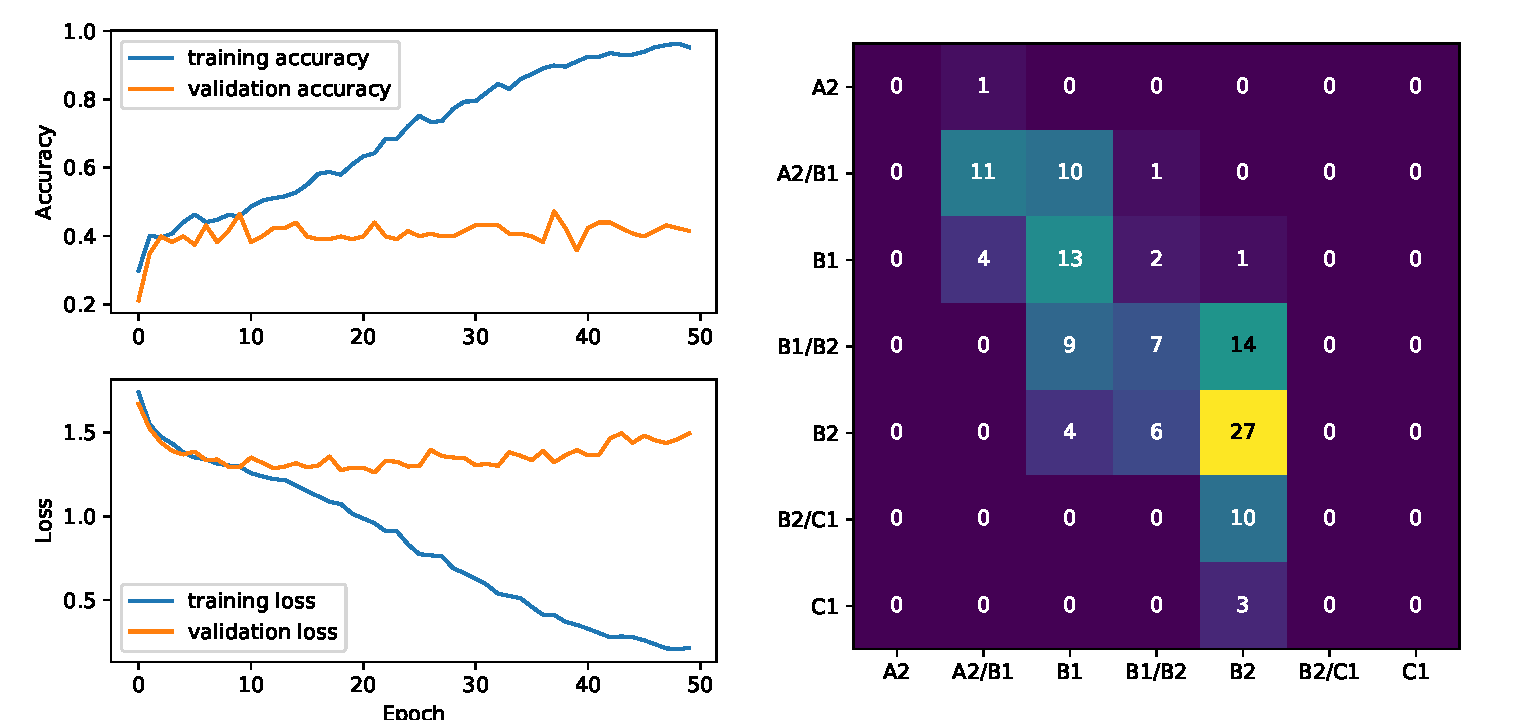
\includegraphics{cnn-training}
    \caption{Training and validation loss and accuracy over 50 epochs of training.}
  \end{subfigure}
  \begin{subfigure}{\linewidth}
    \centering
    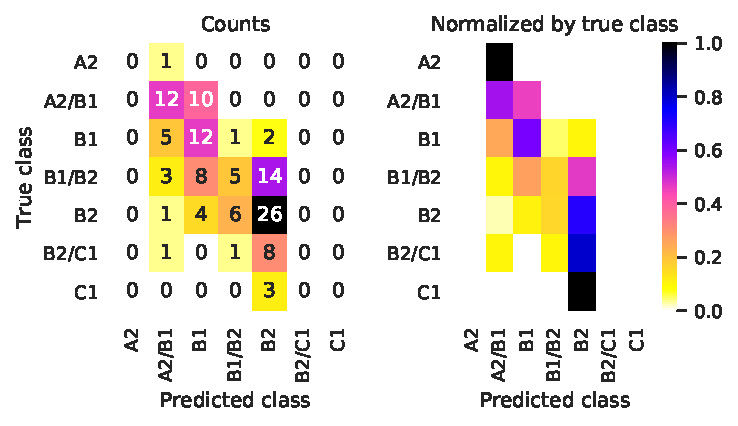
\includegraphics{cnn-confusion}
    \caption{Confusion matrix on validation set, raw counts and normalized.}
  \end{subfigure}
  \caption{CNN with UPOS as side input, using pre-trained, static embeddings.}
  \label{fig:cnn-training}
\end{figure}

Figure \ref{fig:cnn-training} shows that how the training and validation
metrics evolve in the course of training, as well as the confusion matrix of
the final model. The validation metrics plateau after approximately 20
epochs, after which any improvement is eclipsed by small, seemingly random
fluctuations. The training metrics keep improving, suggesting that the model
is memorizing the data rather than discovering general features. When
training stops after 50 epochs, the training accuracy is almost at 100\%.

The confusion matrix reveals that the final model has no predictions for the
classes `A2', `B2/C1' and `C1', the smallest classes in the validation set.


\section{Recurrent neural networks}

Several \ac{RNN} models were implemented based on the architecture described in
\textcite{taghipour16}. Changes to their architecture were made in
order to accommodate our data. For instance, \citeauthor{taghipour16} modelled
the task as a regression problem, their output layer consisting of a single
node with a value constrained to $(0,1)$ by the sigmoid function. This layer
was replaced with a softmax layer similar to the \acp{MLP} in section
\ref{subsec:mlp} and the \acp{CNN} earlier in this chapter.

Having replaced the output layer, we also used a different loss function,
since it needed to be suited for multi-class output. As before, we used
categorical cross-entropy (equation \ref{eq:crossentropy}). A different
evaluation metric was also needed because we are treating the task as
multi-class prediction. We are reporting macro and micro \FI as before. Refer
to section \ref{metrics-discussion} for the discussion of different metrics
for the task.

The formulation of the \ac{AES} task as a regression problem by
\citeauthor{taghipour16} was partly a constraint stemming from the Kaggle
competition that supplied the data and problem formulation, and partly
motivated by the nature of the data. The ASAP data that they use consists of
essays from eight different prompts, and the scoring methods differs across
prompts. Since the scores are numeric values over different ranges, modelling
the task as a regression problem made it sufficient to normalize the numeric
scores to a common interval before training.

Unlike our corpus, ASK, the ASAP dataset used by \citeauthor{taghipour16}
contained essays that were not necessarily written in a second language. Our
data is not split into different parts based on the prompt. There are two
different test levels in ASK, but these are not distinguished in training.

\todo{remainder of section unstructured} Generally for \ac{AES}, modelling
the task as multi-class prediction is common, and is used in
\textcite{vajjala18universalCEFR}. In \textcite{vajjala17}, two different
datasets with different properties were used, and the author utilized both
multi-class prediction and regression at different points. The embedding
layer in \textcite{taghipour16} was initialized with pre-trained embeddings
of size 100.


\subsection{Variants}

We create \acp{RNN} with two different types of gated \ac{RNN} cell, the
\ac{LSTM} and the \ac{GRU}. The concept of gated cells is explained in
section \ref{seq:rnn}, along with the equations defining the gated cells. In
Keras, the default activation function for the gates in gated RNNs is the
\emph{Hard sigmoid} activation function (ref. eq. \ref{eq:hardsigmoid}),
chosen because it is computationally more efficient than the sigmoid
function.

We attempted three different methods of combining the sequence of hidden
states from the \ac{RNN} into a feature vector. The simplest approach is
\emph{mean over time}, where we apply element-wise averaging to the RNN output
across the time dimension. This means that the first element of the
representation vector is the average of the first element of the RNN output
across time, and similarly for the second element, etc.

\[
  \mathrm{mean o/ time}(x_i) = \sum_{t=0}^T o_{t_i}
\]

The second method is similar to the first, except that the averaging
operation is replaced by a max operation. We refer to this as the \emph{max
over time}.

\[
  \mathrm{max o/ time}(x_i) = \max_{t=0}^T o_{t_i}
\]

The final method is an attention layer, which differs from the mean over
time layer in that time steps are weighted by an attention mechanism: a
single-layer neural network computes a value between -1 and 1 for eac
time step. These values are normalized by a softmax layer and then used to
compute the weighted average. Since each time step contributes to the final
representation in differing amounts, the mechanism should be able in theory
to focus on crucial information by choosing weights such as to disregard
uninformative time steps, improving performance. The attention mechanism is
trained along with the rest of the network.

The bidirectional models (BiRNN) are constructed by running two \acp{RNN} over
the same input, but in the opposite order. The output from the BiRNN layer is
a sequence of vectors where, for each time step $j$, the vector is the
concatenation of two vectors $[s_f;s_b]$ where $s_f$ at time step $j$ is the
output from the forwards \ac{RNN} after processing the inputs $(x_1, x_2,
\ldots, x_j)$ and $s_b$ the output from the backwards \ac{RNN} after
processing the inputs $(x_m, x_{m-1}, \ldots, x_j)$, where $m$ is the total
number of time steps. The BiRNN should therefore be able to extract context
on both sides of a input time step.

All the models have a hidden state vector of size 300 in unidirectional
\acp{RNN}, and 600 in BiRNNs (300 in each direction). We use almost all
tokens in the training set as our lexicon, giving a vocabulary size of
20,000. Embeddings are initialized randomly or using vectors from the
fastText model described in section \ref{subseq:fasttext}, and trained as
part of the network.


\section{Results}

The RNN results are split into two tables. Table \ref{tab:lstm-results}
contains the results for models with \ac{LSTM} cells, while table
\ref{tab:gru-results} contains the results for models with \ac{GRU} cells.
The mixed input format is not applicable when using pre-trained embeddings.

\begin{table}
  \centering
  \begin{tabular}{lrrrr}
    \toprule
            & \multicolumn{2}{c}{All labels} & \multicolumn{2}{c}{Collapsed labels} \\
    \cmidrule(lr){2-3}
    \cmidrule(lr){4-5}
    Model     & Macro \FI      & Micro \FI      & Macro \FI      & Micro \FI \\
    \midrule
              \multicolumn{5}{c}{Random init, unidirectional RNN} \\
    \midrule
    % $BEGIN autotable lstm-results
    % $META models-per-row=2 columns-per-model=macrof1,microf1
    % $ROW Mean:        rnn-26285652_1       rnn-26285653_1
    % $ROW Max:         rnn-26285652_2       rnn-26285653_2
    % $ROW Attn.:        rnn-26285652_3       rnn-26285653_3
    % $ROW +POS Mean:   rnn-26285652_4       rnn-26285653_4
    % $ROW +POS Max:    rnn-26285652_5       rnn-26285653_5
    % $ROW +POS Attn:   rnn-26285652_6       rnn-26285653_6
    % $ROW Mix Mean:    rnn-26285652_7       rnn-26285653_7
    % $ROW Mix Max:     rnn-26285652_8       rnn-26285653_8
    % $ROW Mix Attn:    rnn-26285652_9       rnn-26285653_9
    % \midrule \multicolumn{5}{c}{Random init, BiRNN} \\ \midrule
    % $ROW Mean:        rnn-26285652_10      rnn-26285653_10
    % $ROW Max:         rnn-26285652_11      rnn-26285653_11
    % $ROW Attn:        rnn-26285652_12      rnn-26285653_12
    % $ROW +POS Mean:   rnn-26285652_13      rnn-26285653_13
    % $ROW +POS Max:    rnn-26285652_14      rnn-26285653_14
    % $ROW +POS Attn:   rnn-26285652_15      rnn-26285653_15
    % $ROW Mix Mean:    rnn-26285652_16      rnn-26285653_16
    % $ROW Mix Max:     rnn-26285652_17      rnn-26285653_17
    % $ROW Mix Attn:    rnn-26285652_18      rnn-26285653_18
    % \midrule \multicolumn{5}{c}{Pre-trained, unidirectional RNN} \\ \midrule
    % $ROW Mean:        rnn-26287006_19      rnn-26287007_19
    % $ROW Max:         rnn-26287006_20      rnn-26287007_20
    % $ROW Attn:        rnn-26287006_21      rnn-26287007_21
    % $ROW +POS Mean:   rnn-26287006_22      rnn-26287007_22
    % $ROW +POS Max:    rnn-26287006_23      rnn-26287007_23
    % $ROW +POS Attn:   rnn-26287006_24      rnn-26287007_24
    % \midrule \multicolumn{5}{c}{Pre-trained, BiRNN} \\ \midrule
    % $ROW Mean:        rnn-26287006_25      rnn-26287007_25
    % $ROW Max:         rnn-26287006_26      rnn-26287007_26
    % $ROW Attn:        rnn-26287006_27      rnn-26287007_27
    % $ROW +POS Mean:   rnn-26287006_28      rnn-26287007_28
    % $ROW +POS Max:    rnn-26287006_29      rnn-26287007_29
    % $ROW +POS Attn:   rnn-26287006_30      rnn-26287007_30
    % $END autotable
    Mean & $0.265$ & $0.382$ & $0.455$ & $0.675$ \\
    Max & $0.301$ & $0.366$ & $0.562$ & $0.577$ \\
    Attn & $0.240$ & $0.358$ & $0.651$ & $0.748$ \\
    +POS Mean & $0.311$ & $0.415$ & $0.458$ & $0.691$ \\
    +POS Max & $0.362$ & $0.374$ & $0.449$ & $0.659$ \\
    +POS Attn & $0.258$ & $0.374$ & $0.527$ & $0.756$ \\
    Mix Mean & $0.220$ & $0.333$ & $0.384$ & $0.634$ \\
    Mix Max & $0.221$ & $0.374$ & $0.420$ & $0.650$ \\
    Mix Attn & $0.244$ & $0.431$ & $0.485$ & $0.748$ \\
    \midrule \multicolumn{5}{c}{Random init, BiRNN} \\ \midrule
    Mean & $0.343$ & $0.350$ & $0.493$ & $0.715$ \\
    Max & $0.262$ & $0.358$ & $0.606$ & $0.724$ \\
    Attn & $0.288$ & $\mathbf{0.472}$ & $\mathbf{0.674}$ & $0.724$ \\
    +POS Mean & $0.271$ & $0.358$ & $0.485$ & $0.732$ \\
    +POS Max & $0.338$ & $0.382$ & $0.465$ & $0.683$ \\
    +POS Attn & $0.277$ & $0.415$ & $0.548$ & $\mathbf{0.772}$ \\
    Mix Mean & $0.215$ & $0.341$ & $0.414$ & $0.634$ \\
    Mix Max & $0.242$ & $0.366$ & $0.465$ & $0.675$ \\
    Mix Attn & $0.267$ & $0.390$ & $0.480$ & $0.740$ \\
    \midrule \multicolumn{5}{c}{Pre-trained, unidirectional RNN} \\ \midrule
    Mean & $0.291$ & $0.415$ & $0.469$ & $0.675$ \\
    Max & $0.334$ & $0.398$ & $0.450$ & $0.659$ \\
    Attn & $0.358$ & $0.325$ & $0.660$ & $0.732$ \\
    +POS Mean & $0.302$ & $0.423$ & $0.462$ & $0.699$ \\
    +POS Max & $0.353$ & $0.431$ & $0.615$ & $0.732$ \\
    +POS Attn & $0.325$ & $0.415$ & $0.595$ & $0.732$ \\
    \midrule \multicolumn{5}{c}{Pre-trained, BiRNN} \\ \midrule
    Mean & $0.270$ & $0.366$ & $0.464$ & $0.675$ \\
    Max & $0.357$ & $0.350$ & $0.495$ & $0.748$ \\
    Attn & $\mathbf{0.392}$ & $0.350$ & $0.584$ & $0.707$ \\
    +POS Mean & $0.263$ & $0.341$ & $0.472$ & $0.650$ \\
    +POS Max & $0.353$ & $0.455$ & $0.495$ & $0.740$ \\
    +POS Attn & $0.297$ & $0.439$ & $0.637$ & $\mathbf{0.772}$ \\
    \bottomrule
  \end{tabular}
  \caption{\FI scores of LSTM classifiers on AES}
  \label{tab:lstm-results}
\end{table}

\begin{table}
  \centering
  \begin{tabular}{lrrrr}
    \toprule
            & \multicolumn{2}{c}{All labels} & \multicolumn{2}{c}{Collapsed labels} \\
    \cmidrule(lr){2-3}
    \cmidrule(lr){4-5}
    Model     & Macro \FI      & Micro \FI      & Macro \FI      & Micro \FI \\
    \midrule
              \multicolumn{5}{c}{50 dimensional, randomly initialized embeddings} \\
    \midrule
    % $BEGIN autotable gru-results
    % $META models-per-row=2 columns-per-model=macrof1,microf1
    % $ROW Mean:        rnn-26285656_1       rnn-26285657_1
    % $ROW Max:         rnn-26285656_2       rnn-26285657_2
    % $ROW Attn:        rnn-26285656_3       rnn-26285657_3
    % $ROW +POS Mean:   rnn-26285656_4       rnn-26285657_4
    % $ROW +POS Max:    rnn-26285656_5       rnn-26285657_5
    % $ROW +POS Attn:   rnn-26285656_6       rnn-26285657_6
    % $ROW Mix Mean:    rnn-26285656_7       rnn-26285657_7
    % $ROW Mix Max:     rnn-26285656_8       rnn-26285657_8
    % $ROW Mix Attn:    rnn-26285656_9       rnn-26285657_9
    % \midrule \multicolumn{5}{c}{Random init, BiRNN} \\ \midrule
    % $ROW Mean:        rnn-26285656_10      rnn-26285657_10
    % $ROW Max:         rnn-26285656_11      rnn-26285657_11
    % $ROW Attn:        rnn-26285656_12      rnn-26285657_12
    % $ROW +POS Mean:   rnn-26285656_13      rnn-26285657_13
    % $ROW +POS Max:    rnn-26285656_14      rnn-26285657_14
    % $ROW +POS Attn:   rnn-26285656_15      rnn-26285657_15
    % $ROW Mix Mean:    rnn-26285656_16      rnn-26285657_16
    % $ROW Mix Max:     rnn-26285656_17      rnn-26285657_17
    % $ROW Mix Attn:    rnn-26285656_18      rnn-26285657_18
    % \midrule \multicolumn{5}{c}{Pre-trained, unidirectional RNN} \\ \midrule
    % $ROW Mean:        rnn-26287008_19      rnn-26287009_19
    % $ROW Max:         rnn-26287008_20      rnn-26287009_20
    % $ROW Attn:        rnn-26287008_21      rnn-26287009_21
    % $ROW +POS Mean:   rnn-26287008_22      rnn-26287009_22
    % $ROW +POS Max:    rnn-26287008_23      rnn-26287009_23
    % $ROW +POS Attn:   rnn-26287008_24      rnn-26287009_24
    % \midrule \multicolumn{5}{c}{Pre-trained, BiRNN} \\ \midrule
    % $ROW Mean:        rnn-26287008_25      rnn-26287009_25
    % $ROW Max:         rnn-26287008_26      rnn-26287009_26
    % $ROW Attn:        rnn-26287008_27      rnn-26287009_27
    % $ROW +POS Mean:   rnn-26287008_28      rnn-26287009_28
    % $ROW +POS Max:    rnn-26287008_29      rnn-26287009_29
    % $ROW +POS Attn:   rnn-26287008_30      rnn-26287009_30
    % $END autotable
    Mean & $0.293$ & $0.431$ & $0.433$ & $0.650$ \\
    Max & $0.301$ & $0.325$ & $\mathbf{0.668}$ & $0.732$ \\
    Attn & $0.307$ & $0.439$ & $0.536$ & $0.789$ \\
    +POS Mean & $0.277$ & $0.407$ & $0.445$ & $0.683$ \\
    +POS Max & $0.344$ & $0.366$ & $0.439$ & $0.650$ \\
    +POS Attn & $0.308$ & $0.463$ & $0.535$ & $0.772$ \\
    Mix Mean & $0.241$ & $0.398$ & $0.398$ & $0.593$ \\
    Mix Max & $0.272$ & $0.415$ & $0.445$ & $0.707$ \\
    Mix Attn & $0.242$ & $0.431$ & $0.498$ & $0.724$ \\
    \midrule \multicolumn{5}{c}{Random init, BiRNN} \\ \midrule
    Mean & $0.301$ & $0.398$ & $0.473$ & $0.675$ \\
    Max & $0.278$ & $0.301$ & $0.612$ & $0.707$ \\
    Attn & $0.334$ & $0.439$ & $0.492$ & $0.780$ \\
    +POS Mean & $0.281$ & $0.398$ & $0.492$ & $0.683$ \\
    +POS Max & $0.318$ & $0.382$ & $0.448$ & $0.667$ \\
    +POS Attn & $0.366$ & $0.390$ & $0.521$ & $0.740$ \\
    Mix Mean & $0.250$ & $0.358$ & $0.416$ & $0.626$ \\
    Mix Max & $0.259$ & $0.407$ & $0.442$ & $0.683$ \\
    Mix Attn & $0.315$ & $0.415$ & $0.510$ & $0.618$ \\
    \midrule \multicolumn{5}{c}{Pre-trained, unidirectional RNN} \\ \midrule
    Mean & $0.240$ & $0.374$ & $0.462$ & $0.699$ \\
    Max & $0.274$ & $0.382$ & $0.439$ & $0.715$ \\
    Attn & $0.281$ & $0.439$ & $0.524$ & $0.772$ \\
    +POS Mean & $0.271$ & $0.358$ & $0.446$ & $0.699$ \\
    +POS Max & $\mathbf{0.406}$ & $0.407$ & $0.449$ & $0.691$ \\
    +POS Attn & $0.300$ & $0.439$ & $0.509$ & $0.732$ \\
    \midrule \multicolumn{5}{c}{Pre-trained, BiRNN} \\ \midrule
    Mean & $0.293$ & $0.350$ & $0.482$ & $0.715$ \\
    Max & $0.253$ & $0.382$ & $0.460$ & $0.659$ \\
    Attn & $0.345$ & $\mathbf{0.496}$ & $0.543$ & $\mathbf{0.797}$ \\
    +POS Mean & $0.304$ & $0.333$ & $0.459$ & $0.675$ \\
    +POS Max & $0.271$ & $0.366$ & $0.480$ & $0.650$ \\
    +POS Attn & $0.321$ & $0.415$ & $0.513$ & $0.756$ \\
    \bottomrule
  \end{tabular}
  \caption{\FI scores of GRU classifiers on AES}
  \label{tab:gru-results}
\end{table}

We find that many of the best performing models all use the attention
mechanism. Since the stopping criterion for our neural networks is the macro
\FI score, and the micro \FI score is to be considered a side effect of the
macro \FI. In addition there is considerable variance in results between
different training runs of the same model. It is therefore hard to select a
single model as the clear winner. However, it is very unlikely that the best
scores would all be from attention based models by mere chance, and it
therefore seems reasonable to conclude that an attention model is a better
choice for the task than mean over time and max over time.


\subsection{The effect of hyperparameters}

We choose four different hyperparameters and examine the effect each of them
has on the predictions of the networks.


\subsubsection*{Bidirectional RNN}


\subsubsection*{LSTM versus GRU}


\subsubsection*{Initialization of embeddings}


\subsubsection*{UPOS tags}


\subsection{Training behaviour}

\begin{figure}
  % rnn-26287008_27
  \begin{subfigure}{\linewidth}
    \centering
    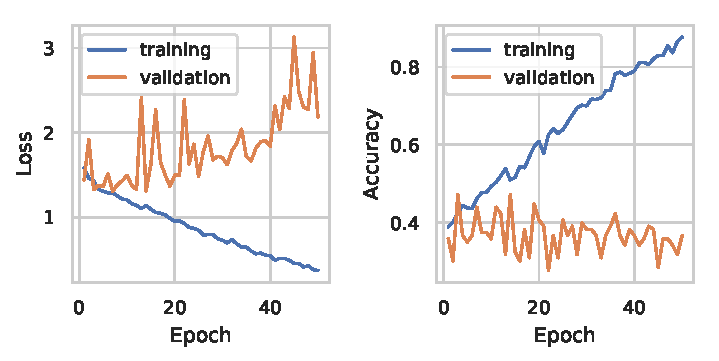
\includegraphics{rnn-training}
    \caption{Training and validation loss and accuracy over 50 epochs of training.}
  \end{subfigure}
  \begin{subfigure}{\linewidth}
    \centering
    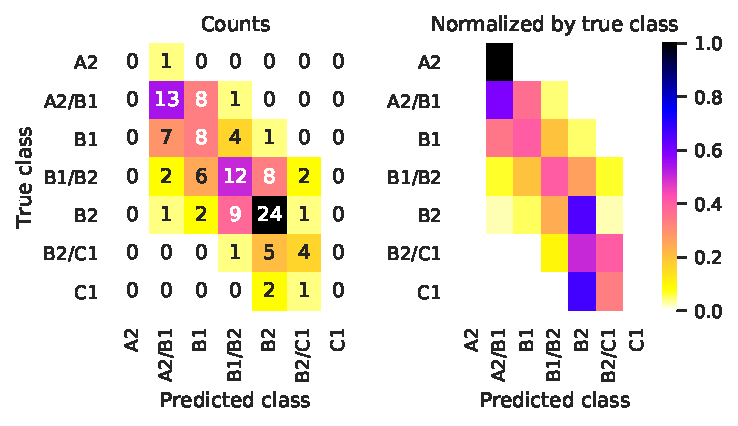
\includegraphics{rnn-confusion}
    \caption{Confusion matrix on validation set, raw counts and normalized.}
  \end{subfigure}
  \caption{BiRNN with GRU cells, attention mechanism, and pre-trained
           embeddings of dimension 100, fine-tuned.}
  \label{fig:rnn-training}
\end{figure}

We see the training and classification of one of the best RNN model in figure
\ref{fig:rnn-training}, a GRU cell with pre-trained, fine-tuned embeddings
and an attention mechanism. The plot of the loss shows that the training loss
decreases in the course of training while the validation loss increases
dramatically. The plot of accuracy over time shows that the validation
accuracy fluctuates around 40\%. While these aspects shows the model
overfitting the training data, the performance on validation data was still
good.

Compared to the training plot of the CNN model in figure
\ref{fig:cnn-training}, it seems that the RNN metrics fluctuate much more,
especially on validation data. However, the training accuracy seems to
increase slower, and does not get as close 100\% in the course of 50 epochs.


\section{Native language identification}

Unlike the proficiency labels in ASK, \ac{L1}s are rather evenly distributed.

We train the same models to classify the documents by native language. The
performance of a \ac{CNN} model improved drastically when including \ac{POS}
tags as input, as evident in table \ref{tab:cnn-nli-results}.

A RNN was able to outperform the CNN only slightly, and here it was not the
attention model that was best, but a bidirectional LSTM.

\begin{table}
  \centering
  \begin{tabular}{lrr}
    \toprule
    Model     & Macro \FI      & Micro \FI \\
    \midrule
    Tokens    &         $0.367$  &         $0.366$  \\ % cnn-nli-2019-02-05_12-54-51
    +POS      & $\mathbf{0.467}$ & $\mathbf{0.463}$ \\ % cnn-nli-2019-01-30_15-32-28
    Mixed POS &         $0.336$  &         $0.333$  \\ % cnn-nli-02-11_16-15-54
    \bottomrule
  \end{tabular}
  \caption{\FI scores of CNN classifiers on NLI}
  \label{tab:cnn-nli-results}
\end{table}

\begin{table}
  \centering
  \begin{tabular}{lrr}
    \toprule
    Model     & Macro \FI      & Micro \FI \\
    \midrule
    Mean/Time &         $0.379$  &         $0.390$  \\ % rnn_nli-25740792
    BiLSTM    & $\mathbf{0.468}$ & $\mathbf{0.480}$ \\ % rnn_nli-25740786
    Attention &         $0.423$  &         $0.407$  \\ % rnn_nli-25740789
    \bottomrule
  \end{tabular}
  \caption{\FI scores of RNN classifiers on NLI}
  \label{tab:rnn-nli-results}
\end{table}


\section{Visualization}

We attempt to use different visualization methods in order to extract
insights about the workings of our models.


\subsection{Attention}

The attention model allows us to visualize the weights the network gives to
each token in a document. In figures
\ref{fig:h0186-nli-attention}--\ref{fig:s0621-nli-attention} we see up to 300
tokens of texts from four different documents in the dev set for which the L1
was correctly predicted by an attention model. Red tokens indicate time steps
that were given higher weight by the attention model, and blue tokens ones
that were given low weights. Out of vocabulary tokens are replaced by the
special token ``UNK''. The attention values do not seem easily interpretable,
as there are lexical and grammatical errors both in the red and the blue
sections.

In the text by an English speaker (fig. \ref{fig:h0189-nli-attention}), one
of the words in a red segment is ``diet'', which the English version of the
intended word (`diett' in Norwegian). The similarity of the words may be a
reason that the writer chose a native form. This is an example of a mistake
that could reveal the writer's \ac{L1}. However, even though this word is
part of a red segment (high attention values), it is not at all certain that
the model actually used it as a clue. The model does not have access to an
English dictionary, so unless the substitution of this very word was a common
pattern among English speakers among our texts, it would have no way to know
that it is actually an English word. Second, `diet' is actually a word form
in Norwegian, meaning `suckle.\textsc{past}'. This is of course a word that
does not fit the context at all.

In the Vietnamese speaker's text (fig. \ref{fig:s0180-nli-attention}), the
word Vietnam appears three times. Two of the occurrences are in
high-attention segments. This should be a very informative word, as it is
likely that when someone mentions a country in this context, it is their
country of origin.

% cspell:disable
In the Somali speaker's text (fig. \ref{fig:s0621-nli-attention}), we see
several typical features of learner language, such as mistakes in agreement:
`en stort rekke hus' should be `et stort rekkehus'. Using a personal pronoun
where there should be a possessive determiner: `faren oss var rik' should be
`faren vår var rik'.
% cspell:enable

\begin{figure}
  \centering
  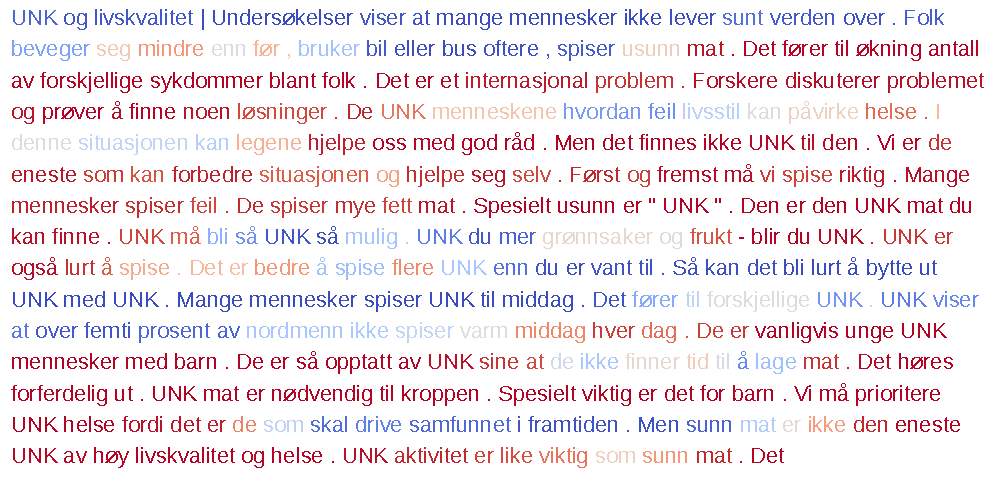
\includegraphics[width=\textwidth]{h0186-nli-attention}
  \caption{Attention values of NLI classifier on excerpt from ASK text h0186.
           L1 is Russian, CEFR score B2}
  \label{fig:h0186-nli-attention}
\end{figure}

\begin{figure}
  \centering
  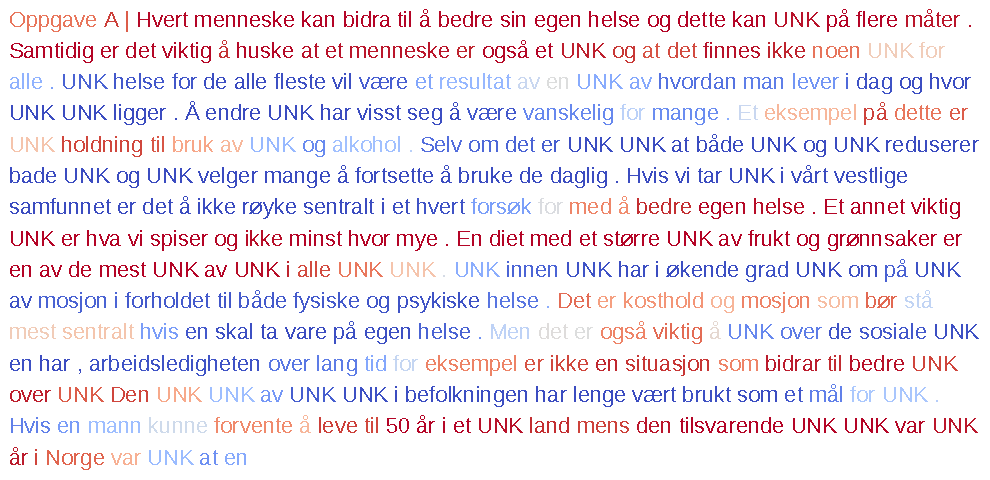
\includegraphics[width=\textwidth]{h0189-nli-attention}
  \caption{Attention values of NLI classifier on excerpt from ASK text h0189.
           L1 is English, CEFR score C1}
  \label{fig:h0189-nli-attention}
\end{figure}

\begin{figure}
  \centering
  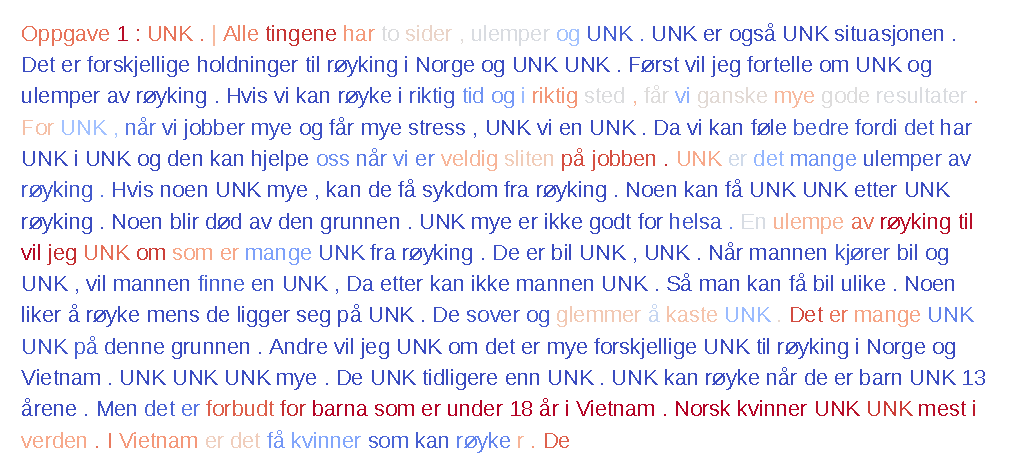
\includegraphics[width=\textwidth]{s0180-nli-attention}
  \caption{Attention values of NLI classifier on excerpt from ASK text s0180.
           L1 is Vietnamese, CEFR score A2/B1}
  \label{fig:s0180-nli-attention}
\end{figure}

\begin{figure}
  \centering
  
\includegraphics[width=\textwidth]{s0621-nli-attention}
  \caption{Attention values of NLI classifier on full ASK text s0621.
           L1 is Somali, CEFR score A2/B1}
  \label{fig:s0621-nli-attention}
\end{figure}
\todo{Visualize UPOS tags}


\subsection{Latent space}

We can use dimensionality reduction methods such as $t$-SNE in order to see
if the intermediate representation of documents prior to the final
classification layer positions documents that should be similar close to each
other. In figure \ref{fig:cefr-t-sne} we have taken the documents in the dev
set and computed these representations using a \ac{CNN}, then run them through
the $t$-SNE algorithm in order to reduce them two two dimensions while still
maintaining a measure of distance. It can be seen that the document space
is split into two clusters, one with generally lower CEFR scores than the
other. However there is no visible structure on a finer level than that.
\todo{use recent model}

\begin{figure}
  \centering
  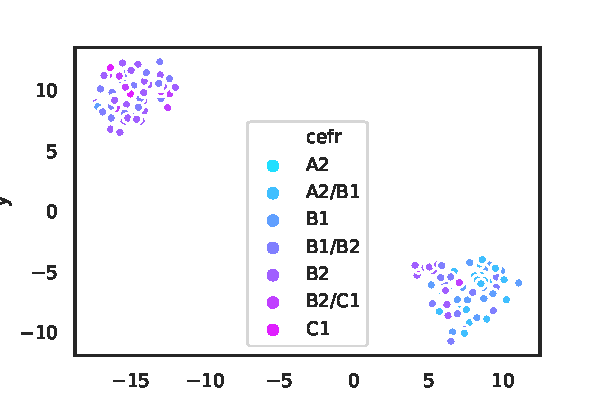
\includegraphics{cefr-t-sne}
  \caption{$t$-SNE plot of the vector representations of documents}
  \label{fig:cefr-t-sne}
\end{figure}
